%%%%%%%%%%%%%%%%%%%%%%%%%%%%%%%%%%%%%%%%%
% Large Colored Title Article
% LaTeX Template
% Version 1.1 (25/11/12)
%
% This template has been downloaded from:
% http://www.LaTeXTemplates.com
%
% Original author:
% Frits Wenneker (http://www.howtotex.com)
%
% License:
% CC BY-NC-SA 3.0 (http://creativecommons.org/licenses/by-nc-sa/3.0/)
%
%%%%%%%%%%%%%%%%%%%%%%%%%%%%%%%%%%%%%%%%%

%----------------------------------------------------------------------------------------
%	PACKAGES AND OTHER DOCUMENT CONFIGURATIONS
%----------------------------------------------------------------------------------------

\documentclass[DIV=calc, paper=a4, fontsize=11pt, twocolumn]{scrartcl}	 % A4 paper and 11pt font size
\usepackage{graphicx} 
\usepackage{lipsum} % Used for inserting dummy 'Lorem ipsum' text into the template
\usepackage[english]{babel} % English language/hyphenation
\usepackage[protrusion=true,expansion=true]{microtype} % Better typography
\usepackage{amsmath,amsfonts,amsthm} % Math packages
\usepackage[svgnames]{xcolor} % Enabling colors by their 'svgnames'
\usepackage[hang, small,labelfont=bf,up,textfont=it,up]{caption} % Custom captions under/above floats in tables or figures
\usepackage{booktabs} % Horizontal rules in tables
\usepackage{fix-cm}	 % Custom font sizes - used for the initial letter in the document
\usepackage[utf8]{inputenc}
\usepackage{sectsty} % Enables custom section titles
\allsectionsfont{\usefont{OT1}{phv}{b}{n}} % Change the font of all section commands

\usepackage{fancyhdr} % Needed to define custom headers/footers
\pagestyle{fancy} % Enables the custom headers/footers
\usepackage{lastpage} % Used to determine the number of pages in the document (for "Page X of Total")

% Headers - all currently empty
\lhead{}
\chead{}
\rhead{}

% Footers
\lfoot{}
\cfoot{}
\rfoot{\footnotesize Page \thepage\ of \pageref{LastPage}} % "Page 1 of 2"

\renewcommand{\headrulewidth}{0.0pt} % No header rule
\renewcommand{\footrulewidth}{0.4pt} % Thin footer rule

\usepackage{lettrine} % Package to accentuate the first letter of the text
\newcommand{\initial}[1]{ % Defines the command and style for the first letter
\lettrine[lines=3,lhang=0.3,nindent=0em]{
\color{DarkGoldenrod}
{\textsf{#1}}}{}}

%----------------------------------------------------------------------------------------
%	TITLE SECTION
%----------------------------------------------------------------------------------------

\usepackage{titling} % Allows custom title configuration

\newcommand{\HorRule}{\color{DarkGoldenrod} \rule{\linewidth}{1pt}} % Defines the gold horizontal rule around the title

\pretitle{\vspace{-30pt} \begin{flushleft} \HorRule \fontsize{50}{50} \usefont{OT1}{phv}{b}{n} \color{DarkRed} \selectfont} % Horizontal rule before the title

\title{\textit{Simulink/Matlab} e Corpos em Queda} % Your article title

\posttitle{\par\end{flushleft}\vskip 0.5em} % Whitespace under the title

\preauthor{\begin{flushleft}\large \lineskip 0.5em \usefont{OT1}{phv}{b}{sl} \color{DarkRed}} % Author font configuration

\author{Fabiano Ap. Marino, } % Your name

\postauthor{\footnotesize \usefont{OT1}{phv}{m}{sl} \color{Black} % Configuration for the institution name
Universidade de São Paulo % Your institution

\par\end{flushleft}\HorRule} % Horizontal rule after the title

\date{} % Add a date here if you would like one to appear underneath the title block

%----------------------------------------------------------------------------------------

\begin{document}

\maketitle % Print the title

\thispagestyle{fancy} % Enabling the custom headers/footers for the first page 

%----------------------------------------------------------------------------------------
%	ABSTRACT
%----------------------------------------------------------------------------------------

% The first character should be within \initial{}
\initial{U}\textbf{m ensaio sobre corpos em queda considerando três casos : queda-livre, queda com força proporcional a resistência do ar e proporcional a 
resistência do ar ao quadrado.}

%----------------------------------------------------------------------------------------
%	ARTICLE CONTENTS
%----------------------------------------------------------------------------------------

\section*{Introdução : \textit{simulink/Matlab}}
Há oque se chama de softwares de linguagem de alto nível, oque significa que há uma grande abstração nos comandos aceitos pelo software, ou seja, os comandos
estão baseados em outros a que são descritos por meio de uma linguagem mais rigida, commo C ou C++, e sua utilização se dá desconsiderando os aspectos dessas
linguagens, tornando mais simples a resolução de muitos problemas. Porém, cabe ressaltar que : apesar do alto nível da linguagem a intenção volta-se a descrever
sistemas de maior complexidade, dificultando assim pelo fenômeno a que se deseja simular, analisar.\\
O simulink, na forma mais simples das linguagens , se utiliza de descrições gráficas para possibilitar a simulação das equações diferenciais que descrevem o fenômeno
tornando a programação simples e agradável, além de que, pessoalmente dizendo, bela e prazerosa.\\
O presente documento tem como intenção a utilização da ferramenta citada na descrição de um simples fenômeno físico : a queda de corpos. Primeiro considera-se 
um corpo em queda livre, sendo que, posteriormente, adiciona-se a resistência do ar considerando-a proporcional a velocidade do corpo e após isto, a consideração
da força de resistência proporcional a velocidade do corpo ao quadrado.\\
As descrições matemáticas dos fenômenos além de sua descrição em blocos simulink é apresentada no documento em questão.

%------------------------------------------------

\section*{Corpo em Queda Livre}
As considerações aqui feitas para o ambiente de queda do corpo são as que se seguem :

\begin{itemize}
 \item Não há resistência do ar : o que signfica que o corpo encontra-se em queda em uma região em que denomina-se vácuo, ou seja, sem a presença de ar, estando
 o mesmo somente atuado pela força peso, de atração gravitacional.
 \item Considera-se também que não há modificações na forma do corpo durante a queda : ou seja, durante a queda, a forma do corpo, a qual influenciaria na força de resistência
 de contra a velocidade, é constante, introduzindo o fato de que a constante de resistência do corpo é constante ao longo de todo o trajeto.
\end{itemize}

Abaixo, encontra-se um desenho do fenômeno em questão, indicando um corpo com a atuação da força peso. Logo mais encontra-se a descrição matemática do mesmo fenômeno.

\begin{figure}[h!]
\centering
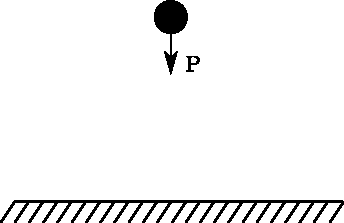
\includegraphics[width=0.5\textwidth]{queda_livre}
\label{fig:queda_livre}
\end{figure}

\newpage

A descrição em termos matemáticos fica como se segue :

\begin{equation}
 \vec{P}=m\frac{d^2\vec{R}}{dt^2}
\end{equation}

A descrição do fenômeno em termos de ambiente simulink fica como se segue, além dos resultados de simulação correspondentes a velocidade e posição do corpo ao
longo do tempo.

\begin{figure}[h!]
\centering
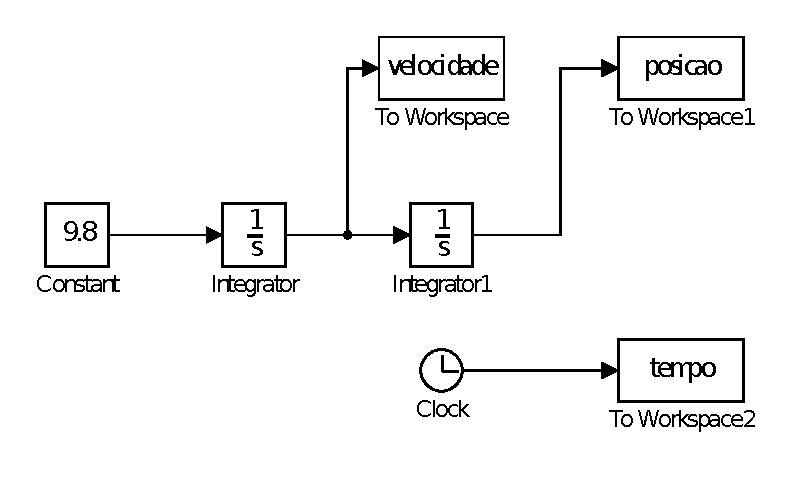
\includegraphics[width=0.4\textwidth]{queda_livre_sem_resistencia_}
\label{fig:queda_livre_sem_resistencia_}
\caption{Descrição em blocos simulinlk}
\end{figure}

\begin{figure}[h!]
\centering
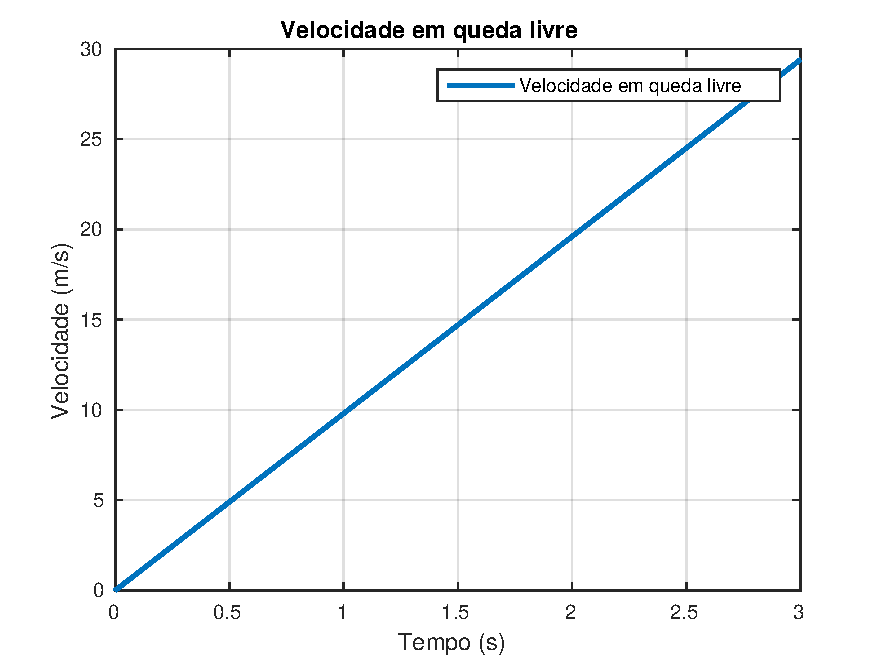
\includegraphics[width=0.4\textwidth]{velocidade_queda_livre}
\label{fig:velocidade_queda_livre}
\caption{Velocidade do bloco em queda livre}
\end{figure}

\begin{figure}[h!]
\centering
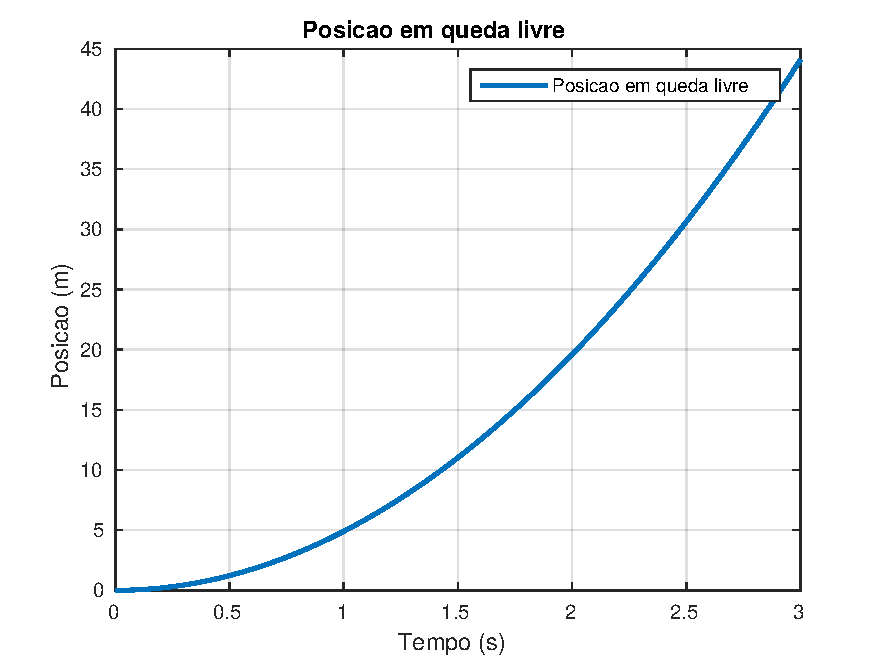
\includegraphics[width=0.4\textwidth]{posicao_queda_livre}
\label{fig:posicao_queda_livre}
\caption{Posição do bloco em queda livre}
\end{figure}

Observa-se que as simulações estão em conformidade com o esperado : a velocidade cresce linearmente, oque é verossímel quanto ao fenômeno em questao, afinal, sobre o
corpo, ao qual atua-se somente a força peso, tem-se como aceleração a da gravidade, fazendo com que a velocidade tenha o comportamento descrito pela equação
$ v(t)= v_{0}+gt $, que nada mais é que uma reta crescente conforme a orientação de $g$. Integrando a velocidade tem-se a posição do corpo no tempo, e é simples a informação
de que a integral de uma equação do primeiro grau é uma do segundo, cujo formato é uma parabola com concavidade segundo as orientações especificadas no fenômeno em questão.
%------------------------------------------------

\newpage

\section*{Queda com força de resistência proporcional a velocidade do ar}
Aqui, passa-se-a a considerar que há uma espécie de fluido no meio ao qual o corpo encontra-se em queda, fazendo com que surja uma resistência a queda devido
ao encontro entre o corpo e as particulas que compõem tal fluido. Primeiramente, como breve elucidação, observa-se o fato de que tal força de resistência é proporcopnal
a velocidade, em uma primeira consideração, e que a mesma tem seu sentido contrário a velocidade do corpo; assim, se o mesmo fosse jogado para cima, a força de resistência
seria para baixo, afinal a velocidade encontra-se para direcionada para cima. O mesmo observa-se para um corpo em queda : estando a velocidade para baixo, a força
de reação ao movimento devido ao meio não vazio de matéria, ou o não vácuo, fará com que a força fique para cima, mais uma vez contrário a velocidade.\\
Mais uma vez a forma do corpo se mantém ao longo do seu movimento, acarretando no fato de que a constante de proporcionalidade de resistência do corpo a queda 
se mantém constante, afinal a mesma mantém relações com a forma do corpo. Afim de melhor elucidar este fato, pensar que uma folha de papel A4, por exemplo, quando
solta ao ar sem estar amassada cai com um comportamento enquanto, se amassada, cai com outro, oque é imaginável para uma grande gama de pessoas que lêm o presente 
documento, mostra a relação entre força de resistência do meio e a forma do corpo. Tudo isto acarreta no fato de que a constante de proporcionalidade de resistência 
mantém, mais uma vez, constante ao longo de todo o movimento, a qual denominar-se-a como sendo \pho.\\
Mas, a força de resistência tem sua expressão dada, tomando o fato de que a mesma é proporcional a constante $\rho$ e a velocidade do corpo, como sendo : $\vec{F_{r}}=\rho \vec{v}$.\\
Desse modo, a expressão que rege o movimento do corpo em queda tem o seguinte formato, além do que, o fenômeno é descrito na figura (\ref{fig:queda_livre_com_resistencia}).
  
\begin{equation}
 +\vec{P}-\rho \vec{v}=m\frac{d^2\vec{R}}{dt^2}
\end{equation}

\begin{figure}[h!]
\centering
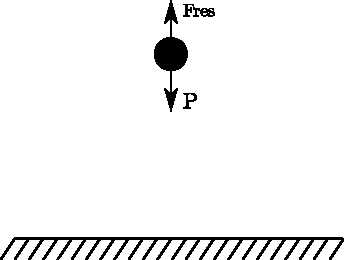
\includegraphics[width=0.4\textwidth]{queda_livre_com_resistencia}
\caption{Diagrama de forças de um corpo em queda com resistência do meio.}
\label{fig:queda_livre_com_resistencia}
\end{figure}

\newpage

Os resultados, bem como a construção em ambiente simulink encontram-se a seguir, expressando resultados concisos e esperados com relação a velocidade e posição
do corpo ao longo do tempo.

\begin{figure}[h!]
\centering
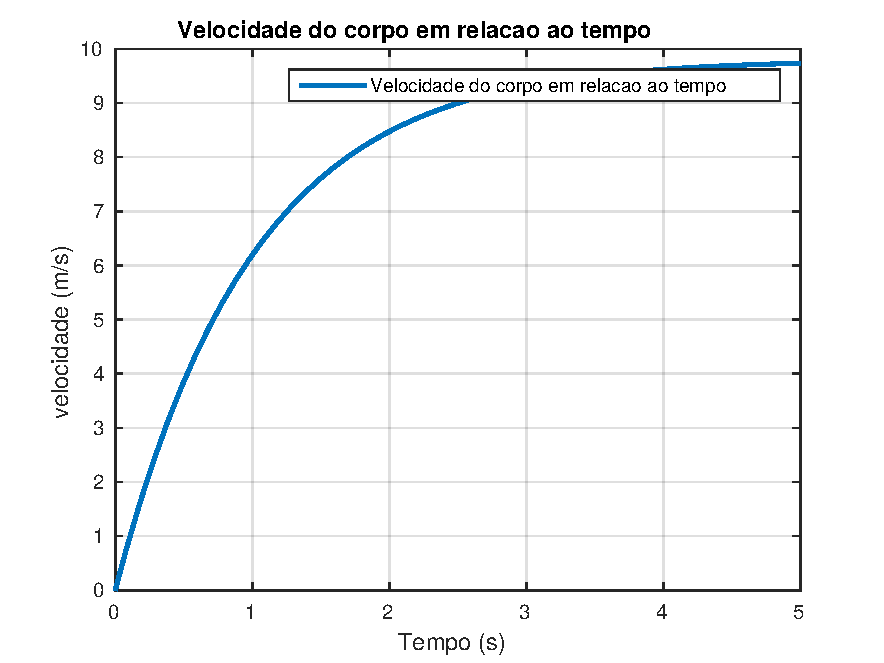
\includegraphics[width=0.4\textwidth]{velocidade}
\caption{Velocidade do corpo com relação ao tempo.}
\label{fig:velocidade}
\end{figure}

\begin{figure}[h!]
\centering
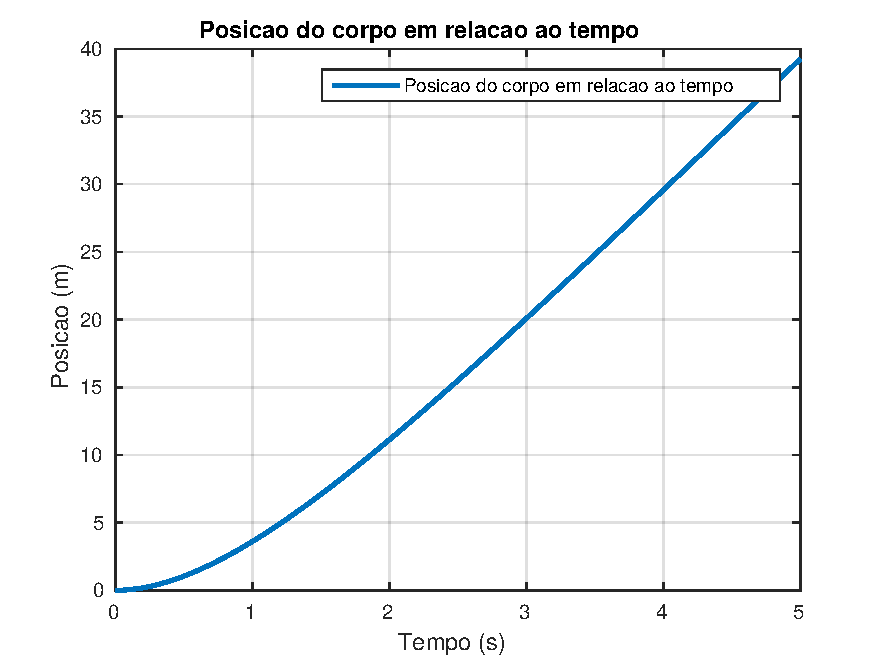
\includegraphics[width=0.4\textwidth]{posicao}
\caption{Posição do corpo com relação ao tempo.}
\label{fig:posicao}
\end{figure}

\newpage

\begin{figure}[h!]
\centering
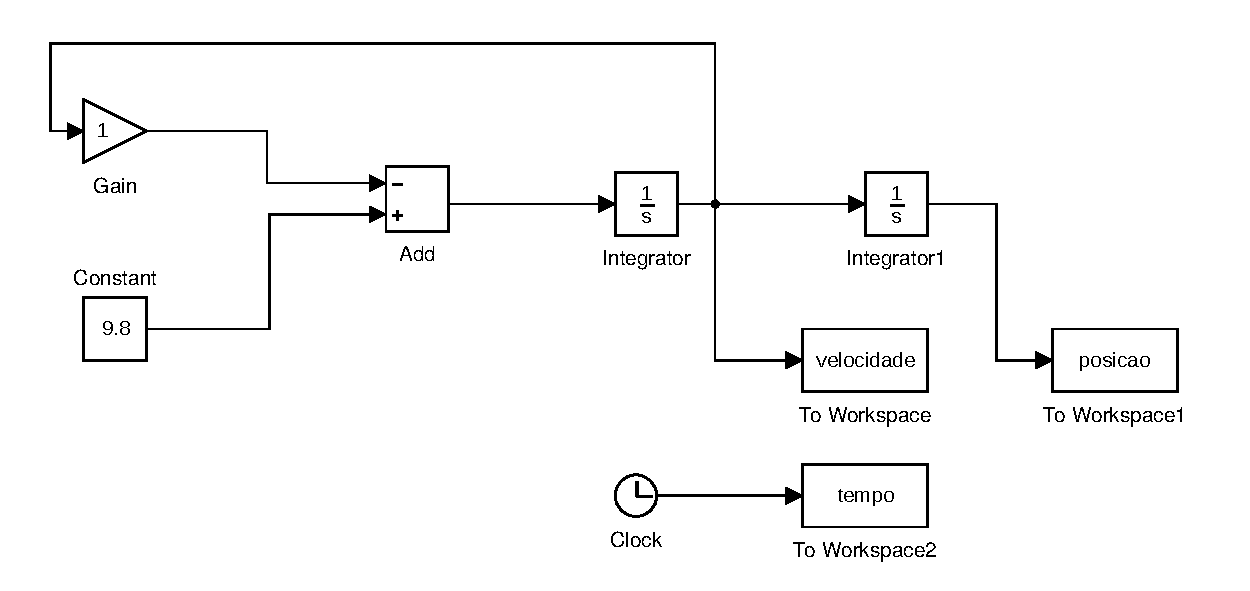
\includegraphics[width=0.5\textwidth]{blocos}
\caption{Construção em blocos do em diagrama simulink.}
\label{fig:blocos}
\end{figure}

O próximo objetivo é simular e descrever um corpo em queda com força de resistência proporcional a velocidade ao quadrado, oque inclui uma não linearidade no
problema.

\section*{Corpo em Queda com Força de Resistência Proporcional a Velocidade do Ar ao Quadrado}
Considera-se agora, o corpo em queda, assim como representado na figura (\ref{fig:queda_livre_com_resistencia}), porém com força de resitência do ar proporcional a velocidade ao quadrado.\\
O equacionamento do fenômeno fica como se segue e os resultados obtidos com relação ao ambiente simulnk fica como se segue nas imagens apresentadas.

\begin{equation}
 \vec{P}-\vec{F}_{res}=m\frac{d^2\vec{R}}{dt^2}
\end{equation}

Implicado em, devido a força de resistência ser proporcional a velocidade ao quadrado :

\begin{equation}
 \vec{P}-m({\frac{d\vec{R}}{dt}})^2=m\frac{d^2\vec{R}}{dt^2}
\end{equation}

Da qual a descrição em ambiente simulink fica como se segue na figura (\ref{fig:blocos_ao_quadrado}) além das simulações referentes a velocidade e deslocamento do corpo presentes nas
figuras (\ref{fig:velocidade_quadrado}) e (\ref{fig:posicao_do_corpo_ao_quadrado}).

\begin{figure}[h!]
\centering
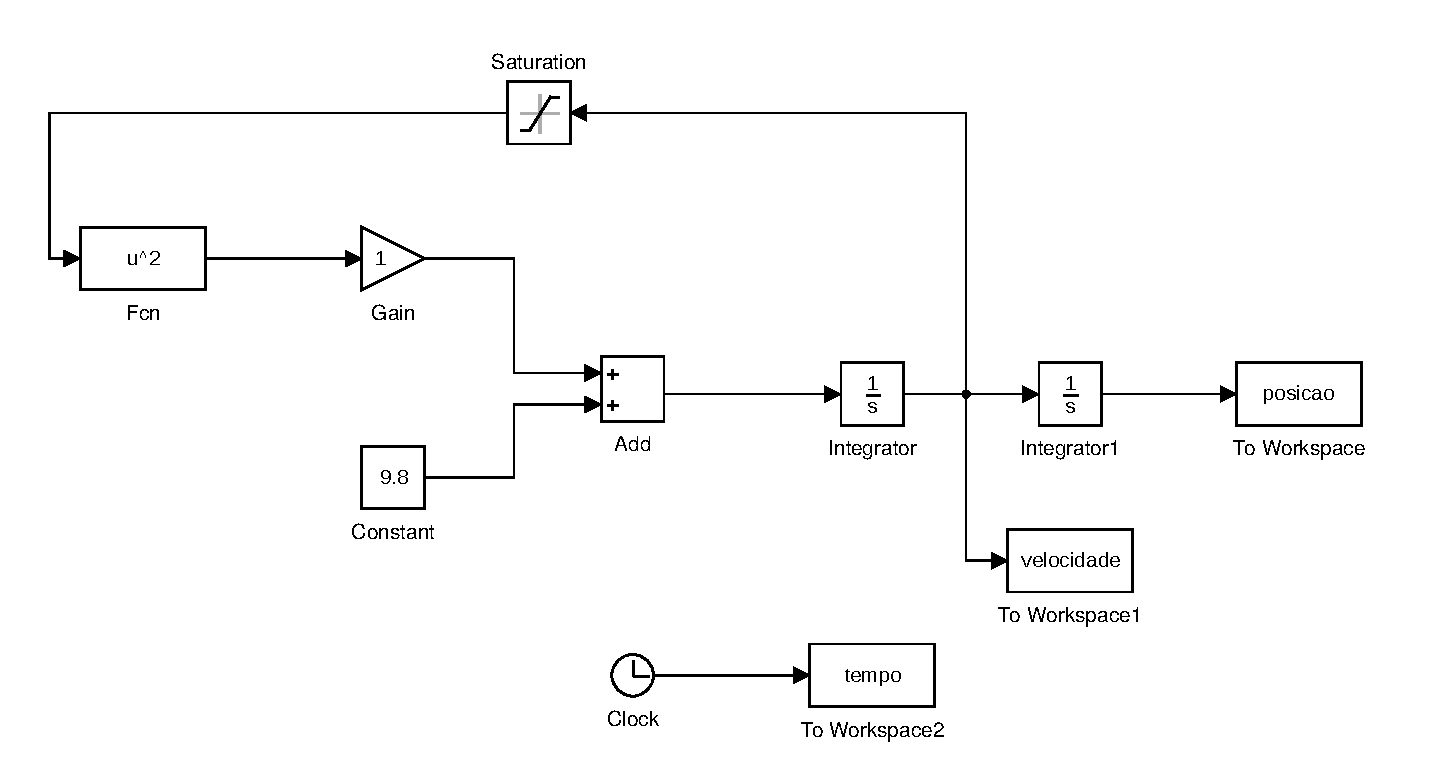
\includegraphics[width=0.4\textwidth]{blocos_ao_quadrado}
\caption{Descrição Simulink com Força de Resistência Proporcional a Velocidade ao Quadrado.}
\label{fig:blocos_ao_quadrado}
\end{figure}

\begin{figure}[h!]
\centering
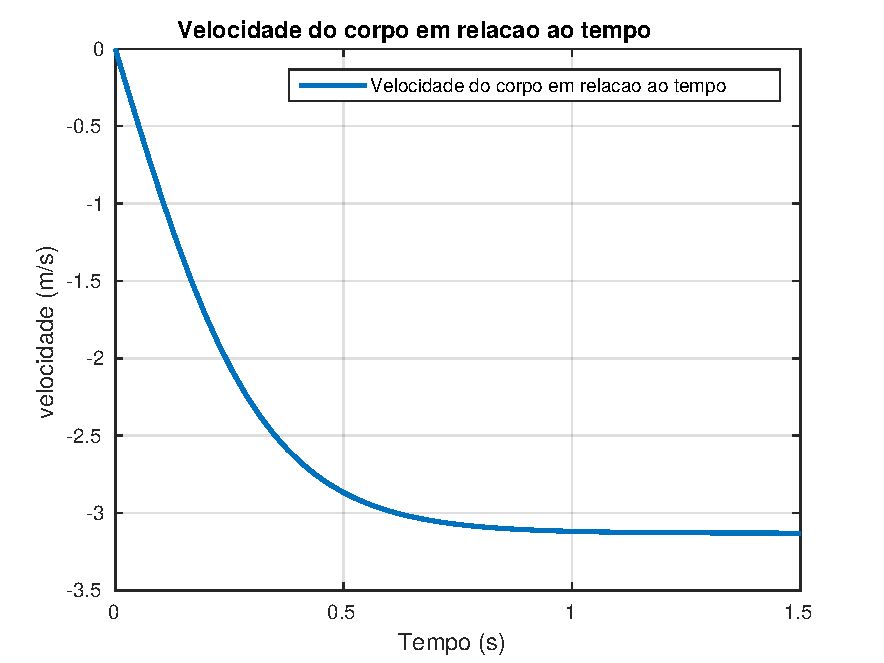
\includegraphics[width=0.5\textwidth]{velocidade_quadrado}
\caption{Velocidade do corpo com relação ao tempo.}
\label{fig:velocidade_quadrado}
\end{figure}

\newpage

\begin{figure}[h!]
\centering
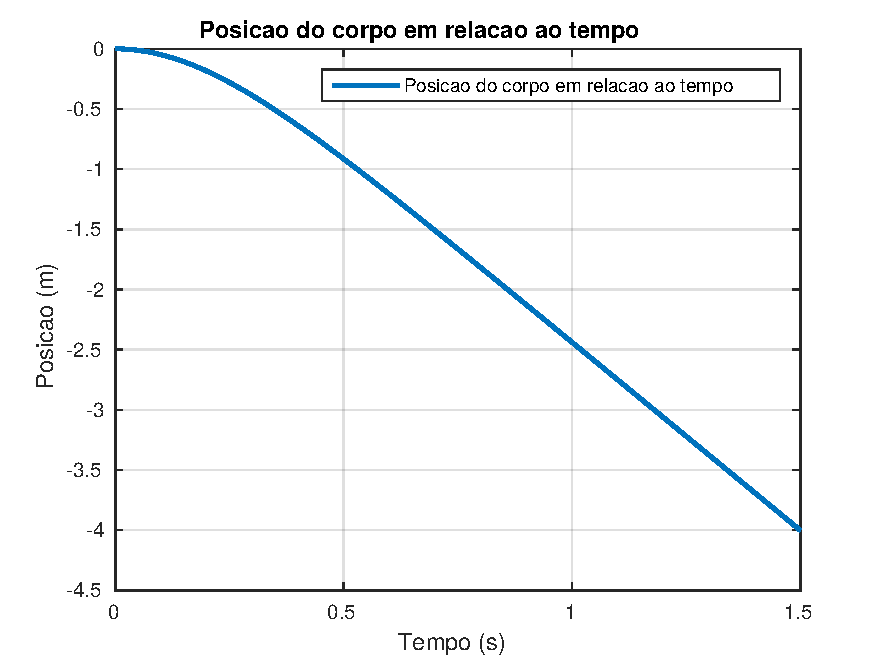
\includegraphics[width=0.5\textwidth]{posicao_do_corpo_ao_quadrado}
\caption{Posição do Corpo com Relação ao tempo.}
\label{fig:posicao_do_corpo_ao_quadrado}
\end{figure}

%----------------------------------------------------------------------------------------
%	REFERENCE LIST
%----------------------------------------------------------------------------------------
\begin{thebibliography}{99} % Bibliography - this is intentionally simple in this template

\bibitem[Moysés Nussveig, 2009]{}
\newblock Curso de Física 1 : Conteúdo Básico
\newblock {\em IFSC}
 
\end{thebibliography}


%----------------------------------------------------------------------------------------

\end{document}